%!TEX root = ../IntrusionResponse.tex

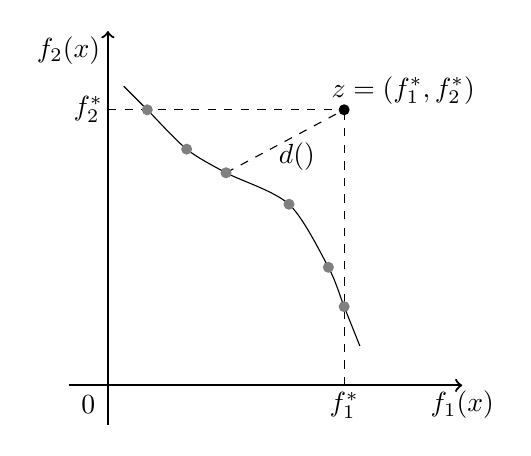
\begin{tikzpicture}
  %\draw (0, 0) to[grid with coordinates] (14, 10);
  \draw[thick,->] (0,-0.5) -- (0,4.5);
  \draw[thick,->] (-0.5,0) -- (4.5,0);
  \node (origin) at (-0.25,-0.25) {0};
  \node (xlabel) at (4.5,-0.25) {$f_1(x)$};
  \node (ylabel) at (-0.5,4.25) {$f_2(x)$};

  \draw plot[smooth] coordinates {(0.2,3.8) (0.5,3.5) (1.0,3.0) (1.5,2.7) (2.3,2.3) (2.8,1.5) (3.0,1.0) (3.2,0.5)};
  \draw[dashed] (0.0,3.5) -- (3.0,3.5);
  \draw[dashed] (3.0,0.0) -- (3.0,3.5);
  \draw[dashed] (1.5,2.7) -- (3.0,3.5);
  \node (disdemo) at (2.4,2.9) {$d()$};

  \fill[gray] (0.5,3.5) circle (2pt);
  \fill[gray] (1.0,3.0) circle (2pt);
  \fill[gray] (1.5,2.7) circle (2pt);
  \fill[gray] (2.3,2.3) circle (2pt);
  \fill[gray] (2.8,1.5) circle (2pt);
  \fill[gray] (3.0,1.0) circle (2pt);

  \fill[black] (3.0,3.5) circle (2pt);
  \node (idealoptimal) at (3.75,3.75) {$z = (f_1^*,f_2^*)$};
  \node (yoptimal) at (-0.25,3.5) {$f_2^*$};
  \node (xoptimal) at (3.0,-0.25) {$f_1^*$};

\end{tikzpicture}